\newpage
\appendix

\chapter{Example of deploying an IOC with YAML file}
An example YAML file used to deploy \gls{IOC}. In this particular case, the IOC operated a BINDER MK240 climatic chamber~\cite{binder} using Modbus protocol~\cite{modbus}. The volumes are used to acquire database files and synchronize the time with the node. The container is deployed in the host network and the so-called pseudo-terminal is activated (tty). The time of the container is synchronized with the local time of the node. 
\label{YAML}
\begin{verbatim}

version: "3.7"
services:
  binder:
    container_name: binderioc
    volumes:
      - "/home/cbm/dcs-sts/config/:/config"
      - "/etc/localtime:/etc/localtime:ro"
      - "/etc/timezone:/etc/timezone:ro"
    network_mode: "host"
    image: "paluma.rub.de/panda-ioc"
    tty: true
    command: /config/iocBoot/iocBinder/st.cmd
\end{verbatim}

\chapter{CSA scans for modules of the mSTS}
\label{CSA}
The graphs depict the current trends of the \gls{STS} modules in the function of the CSA value settings. The nominal operational value of 31 value is also marked. The respective components that cause higher average current for Unit 1 and 3 are listed in Chapter 6. The newest modules which are in the Unit 2 present similar currents as Unit 0. 
\vfill
\begin{figure}[h!]
\centering
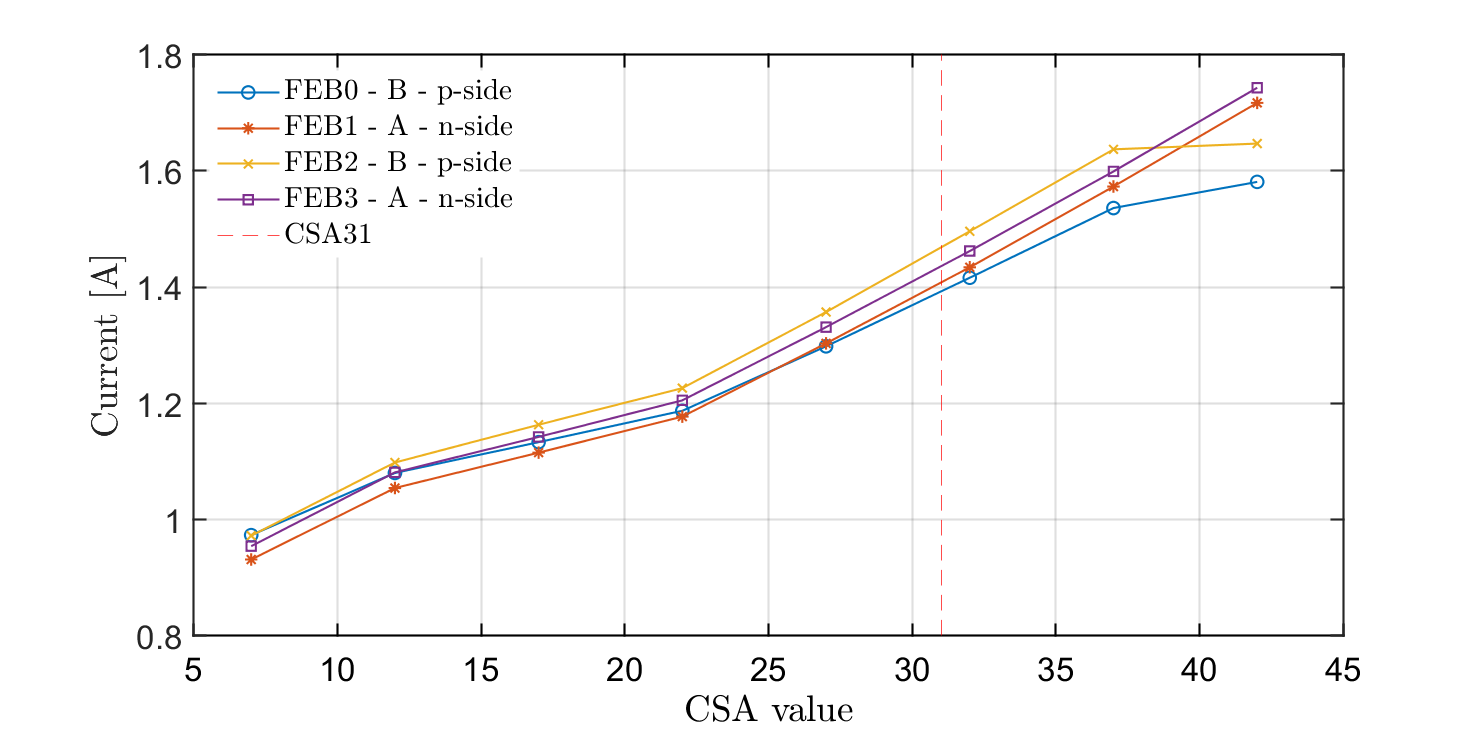
\includegraphics[width=0.9\columnwidth]{Chapter6/DCS/images/U1CSABIAS.png}
\caption{Currents of four \glspl{FEB} of Unit 1 in function of CSA value setting.}
\label{U1CSABIAS}
\end{figure}
\vfill
\begin{figure}
\centering
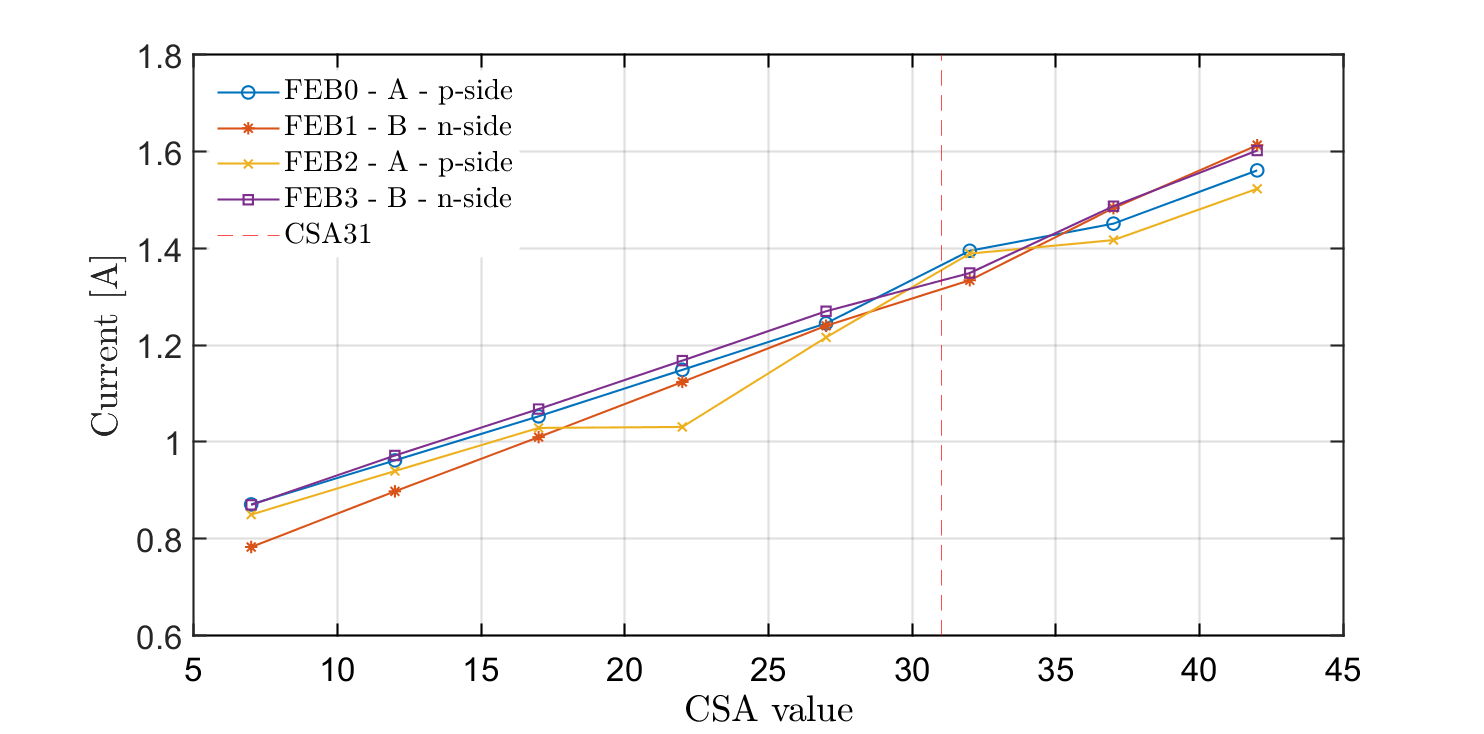
\includegraphics[width=0.9\columnwidth]{Chapter6/DCS/images/U2CSABIAS.png}
\caption{Currents of four \glspl{FEB} of Unit 2 in function of CSA value setting.}
\label{U2CSABIAS}
\end{figure}

\begin{figure}[h!]
\centering
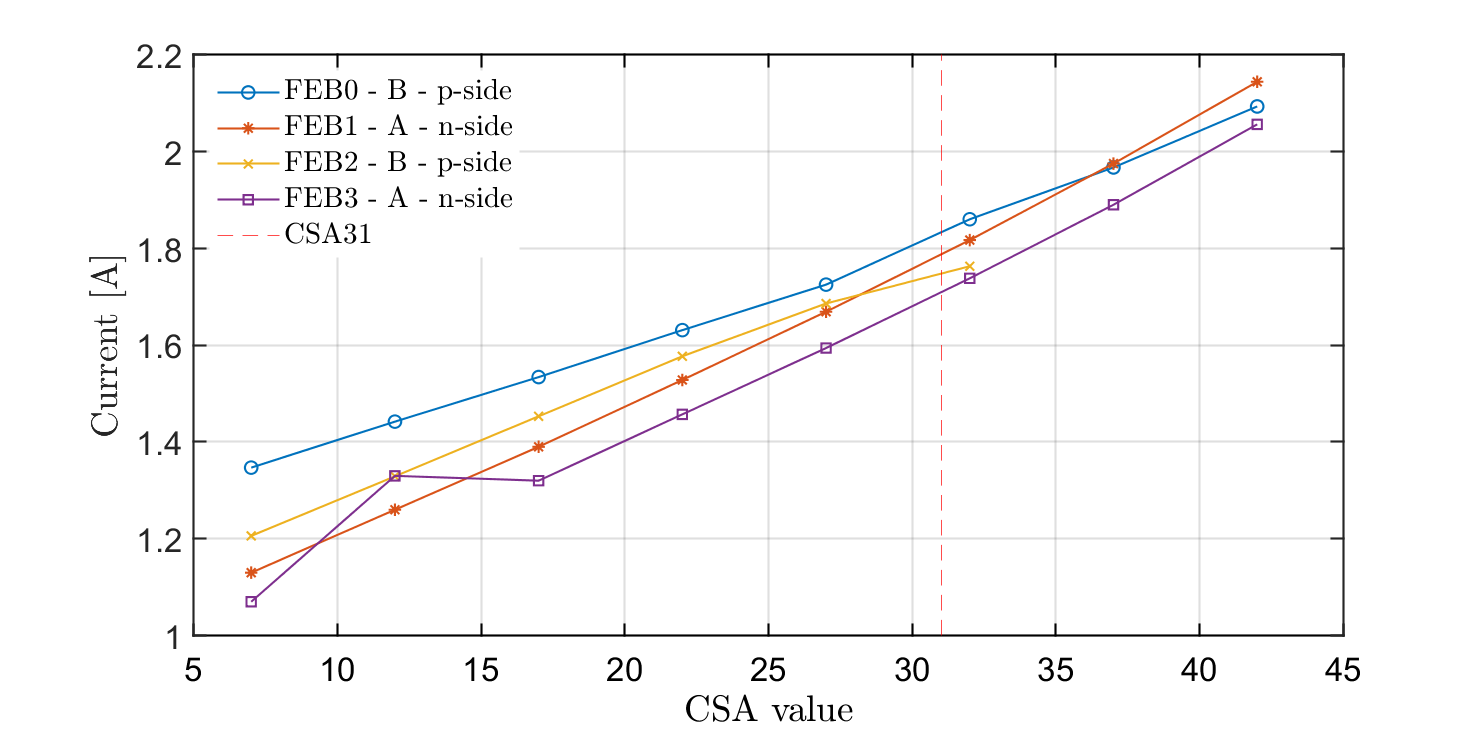
\includegraphics[width=0.9\columnwidth]{Chapter6/DCS/images/U3L1CSABIAS.png}
\caption{Currents of four \glspl{FEB} of Unit 3 Ladder 0 in the function of CSA value settings.}
\label{U3L1CSABIAS}
\end{figure}

\chapter{Leakage current evolution}
\label{Current}
Figures~\ref{leakage_current_u1u2} and \ref{leakage_current_u3l1} depict the leakage current evolution of the remaining \gls{mSTS} modules. Leakage current trends of Unit 1, 2, and module 1 of Unit 3 Ladder 3 are in agreement. Module 0 of Unit 3 is most likely an electrical issue that reveals itself in unusually high leakage current increase. 
\begin{figure}[h!]
\centering
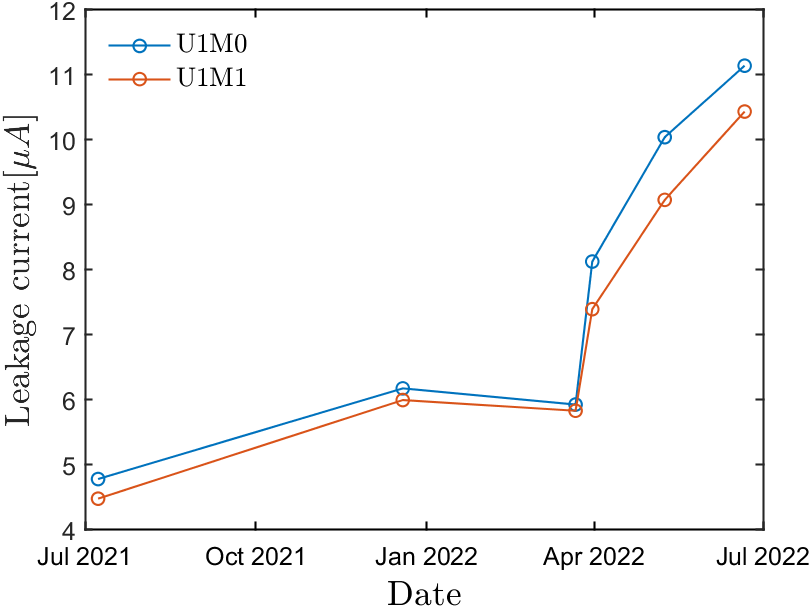
\includegraphics[width=0.47\columnwidth]{Chapter6/DCS/images/sensors/U1_leakage.png}
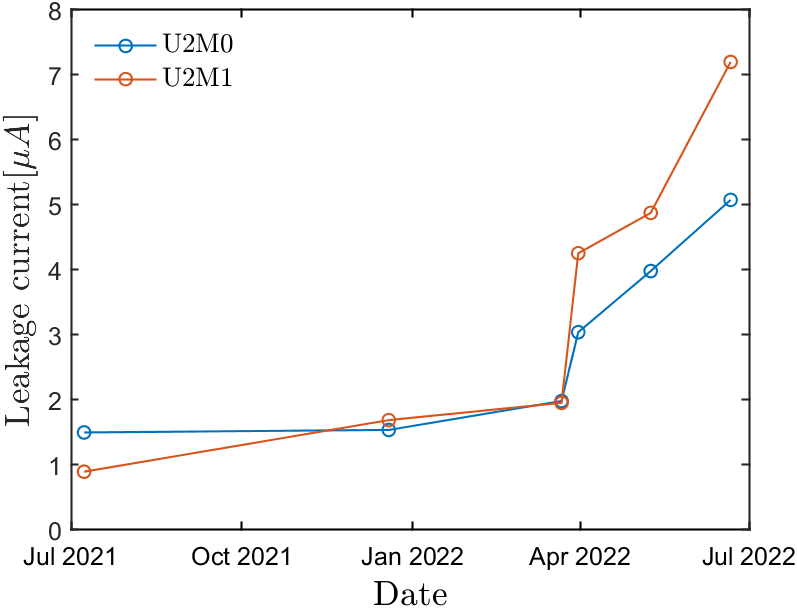
\includegraphics[width=0.47\columnwidth]{Chapter6/DCS/images/sensors/U2_leakage.png}
\caption{Leakage current evolution during the \gls{mSTS} operation - Unit 1 and unit 2.}
\label{leakage_current_u1u2}
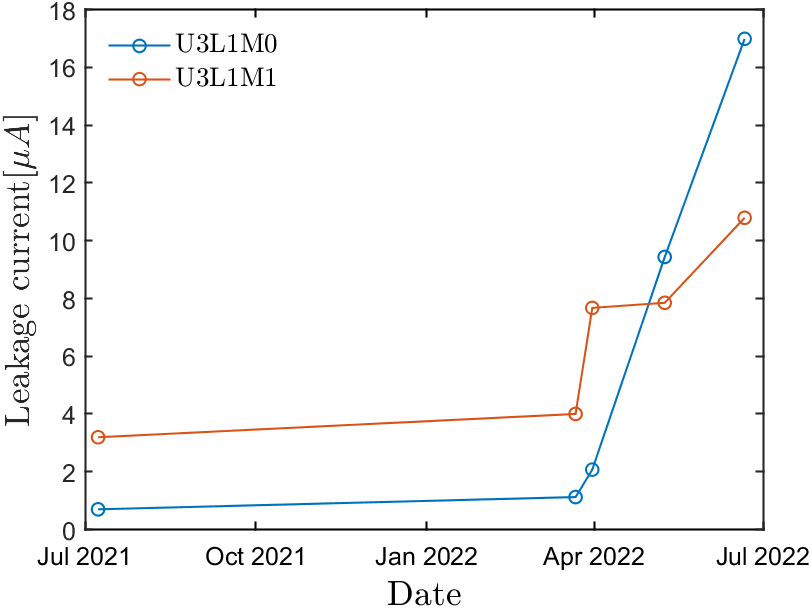
\includegraphics[width=0.5\columnwidth]{Chapter6/DCS/images/sensors/U3L1_leakage.png}
\caption{Leakage current evolution during the \gls{mSTS} operation - Unit 3 ladder 1.}
\label{leakage_current_u3l1}
\end{figure}


%\chapter{IV curves}
%\label{IV}

